%!TEX root = bachelor.tex
\chapter{Theoretische Grundlagen}
\label{ch:theory}

Rechtshändiges Koordinatensystem...

\section{Kegel}
\label{s:cone}

\begin{definition}[Kegel]
	kegel
	$S$ bezeichnet die Seitenhöhe und ist definiert durch $S = \sqrt{H^2 + R^2}$
	$S >= R$ Dreiecksungleichung
\end{definition}

In der weiteren Arbeit betrachten wir nur gerade Kreiskegel

\begin{figure}[!htb]
	\centering
	\includegraphics[scale=.5]{images/fullCone.eps}
	\caption{Gerader Kreiskegel}
	\label{fig:cone}
\end{figure}

Ein Kegel mit Spitze $T(0,0,0)$, Radius $R$ und Höhe $H$ kann parametrisch beschrieben werden als:
\begin{equation}
\begin{aligned}
x &= \frac{u}{h} R~cos \theta \\
y &= u \\
z &= \frac{u}{h} R~sin \theta
\end{aligned}
\end{equation}
mit $u\in [0, H]$ und $\theta \in [0, 2\pi)$ 


\begin{definition}[Kegelstumpf und Ergänzungskegel]
	Ein Kegelstumpf entsteht als Schnitt eines geraden Kreiskegels mit einer zur Grundfläche parallelen Ebene (siehe Abbildung \ref{fig:coneWithFrustum}). Das Stück von Grundfläche zur Schnittfläche nennen wir Kegelstumpf. Die Differenz zum eigentlichen Kegel wird als Ergänzungskegel bezeichnet. 
	
	$H, R, S$ bleiben die Angaben des gesamten Kegels. Hinzu kommen $h,r,s$ als Angaben des Ergänzungskegels. Die Höhe, sowie die Seitenhöhe des Kegelstumpfs werden durch die Differenzen $\Delta S = S - s,~ \Delta H = H-h$ charakterisiert (siehe Abbildung \ref{fig:coneFrustum}).
\end{definition}

\begin{figure}[!htb]
	\centering
	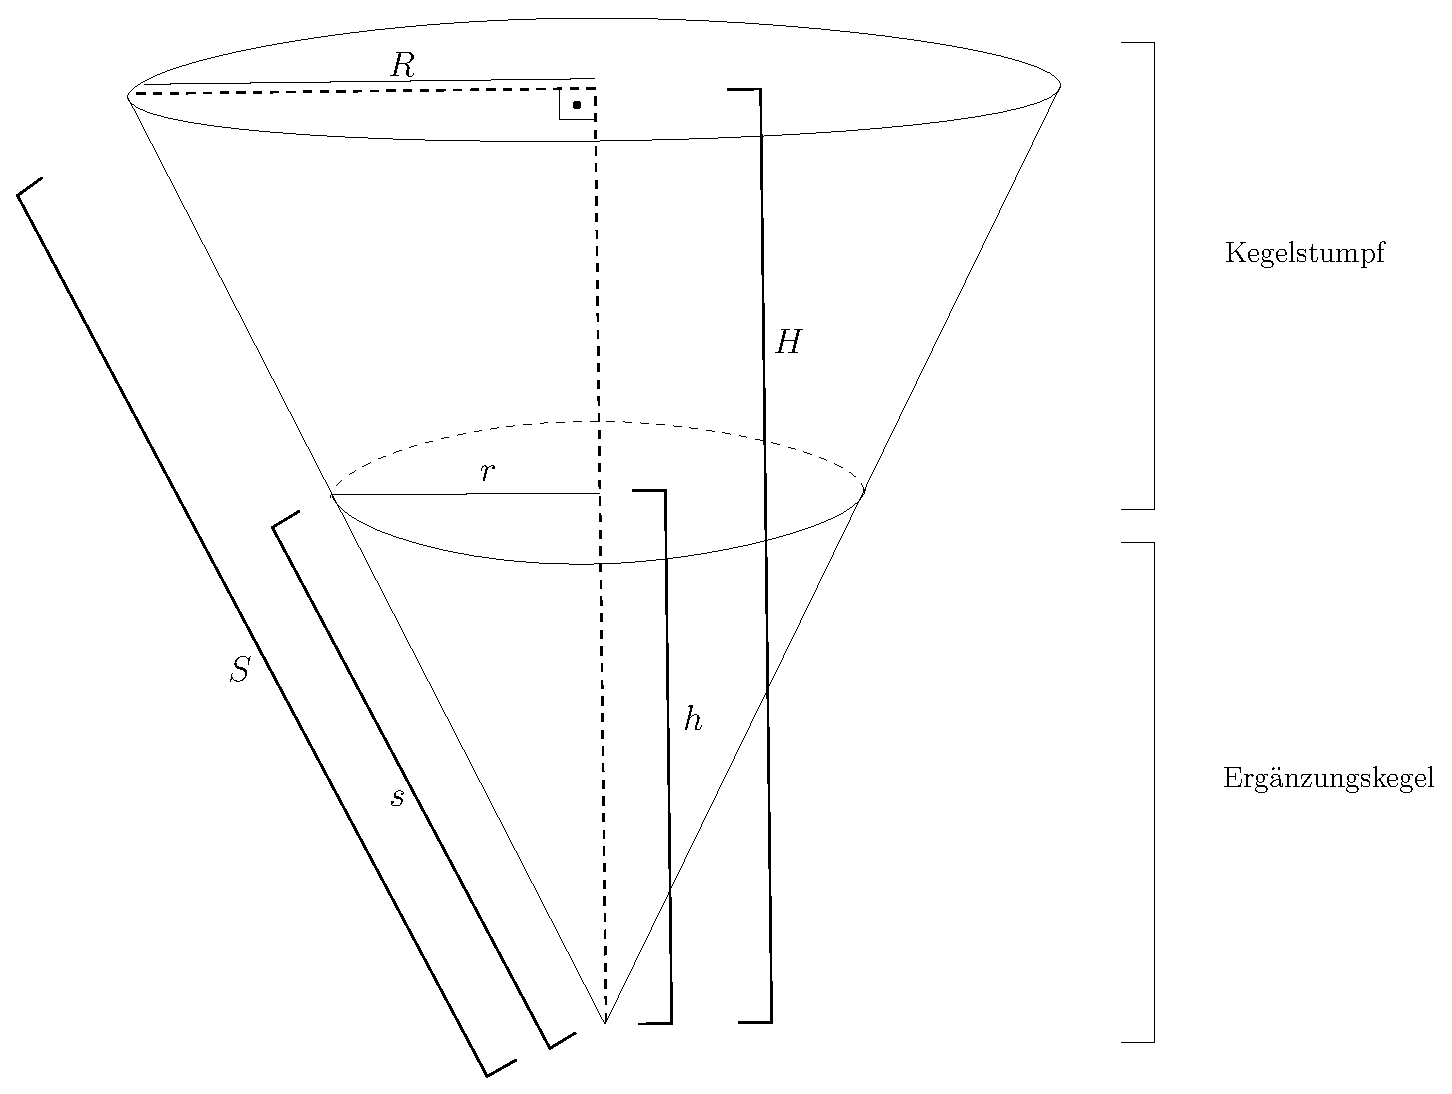
\includegraphics[scale=.5]{images/fullCone3.eps}
	\caption{Kegelstumpf und Ergänzungskegel}
	\label{fig:coneWithFrustum}
\end{figure}

\begin{figure}[!htb]
	\centering
	\includegraphics[scale=.7]{images/coneFrustum.eps}
	\caption{Kegelstumpf}
	\label{fig:coneFrustum}
\end{figure}

Analog zum Kreiskegel definieren wir einen Kegelstumpf durch folgende Parametrisierung: 
\begin{equation} \label{eq:paramFrustum}
\begin{aligned}
x &= (r + \frac{u}{\Delta H} (R - r))~cos \theta \\
y &= u \\
z &= (r + \frac{u}{\Delta H} (R - r))~sin \theta
\end{aligned}
\end{equation}
mit $u\in [0, \Delta H]$ und $\theta \in [0, 2\pi)$


\begin{figure}[!htb]
	\centering
	\includegraphics[scale=.4]{images/coneLateral.eps}
	\caption{Kegelmantelfläche}
	\label{fig:coneLateral}
\end{figure}

Die Mantefläche des Kegelstumpfes aus Abbildung \ref{fig:coneLateral} kann dann parametrisch beschrieben werden als:
\begin{equation} \label{eq:paramLateral}
\begin{aligned}
x &= -(s + \frac{u}{\Delta H}(S-s)) ~sin \phi \\
y &= (s + \frac{u}{\Delta H} (S-s)) ~cos \phi
\end{aligned}
\end{equation}
mit  $u\in [0, \Delta H]$ und $\phi \in [0, \alpha] \subseteq [0, 2\pi]$ mit $\alpha S = 2\pi R \implies \alpha = 2\pi\frac{R}{S}$


Ein Punkt auf der Oberfläche des Kegelstumpfs kann eindeutig einem Punkt auf der Mantelfläche (und umgekehrt) zugeordnet werden. Dazu konstruieren wir folgende Abbildung und ihr Inverses:

Sein ein Punkt $C(x,y,z)$ auf der Oberfläche des Kegelstumpfs gegeben. Wir wissen aus der parametrischen Form \ref{eq:paramFrustum}, dass $C$ die Form
\[
C(x,y,z) = (r + \frac{u}{\Delta H} (R - r))~cos \theta, u, (r + \frac{u}{\Delta H} (R - r))~sin \theta
\]  für ein $u\in [0, \Delta H]$ und $\theta \in [0, 2\pi)$ besitzt. 

Aus der $y$-Koordinate kann man als die Höhe ablesen und somit den Radius in der Mantelfläche als lineare Interpolation zwischen $s$ und $S$ bestimmen (siehe Abbildung \ref{fig:mapToLateralS}). Wir definieren uns hierfür eine Hilfsfunktion 
\begin{equation} \label{eq:Sigma}
	\Sigma(y) := s + \frac{y}{\Delta H} (S-s)
\end{equation}


\begin{figure}[!htb]
	\centering
	\includegraphics[scale=.7]{images/mapToLateralS.eps}
	\caption{Abbildung der Kegelstumpfhöhe auf die Seitenhöhe}
	\label{fig:mapToLateralS}
\end{figure}

Da $R, r, \Delta H$  und nun auch die Höhe bekannt sind, kann man den Winkel $\theta$ im Kegelstumpf einfach ausrechnen. Anschließend muss dieser noch mit  $\frac{R}{S}$ multipliziert werden um ihn auf $[0, \alpha]$ zu skalieren (siehe \ref{eq:paramLateral}).  Auch hierfür definieren wir eine Hilfsfunktion:
\begin{equation*}
\Phi(x,y,z) := \frac{R}{S} \atant\left(\frac{z}{r + \frac{y}{\Delta h} (R - r)}, \frac{x}{r + \frac{y}{\delta H} (R - r)}\right)
\end{equation*}

, wobei wir $\atant$ benutzen um den Winkel im richtigen Quadranten, also in $[0, 2\pi)$, bestimmen zu können. 

Mit diesen beiden Hilfsfunktionen und \ref{eq:paramLateral} ergibt sich insgesamt:
\begin{equation}
\begin{aligned}
\Psi \colon [r,R] \times [0, \Delta H] \times [r,R] &\to [s,S] \times [s,S]\\
\begin{pmatrix}
x \\ y \\ z
\end{pmatrix}  &\mapsto
\begin{pmatrix}
-\Sigma(y)\sin \Phi(x,y,z)\\
 \Sigma(y)\cos\Phi(x,y,z)
\end{pmatrix}
\end{aligned}
\end{equation}

Analog lässt die sich Umkehrabbildung konstruieren:

Sein ein Punkt $L(x,y)$ auf der Mantelfläche des Kegelstumpfs gegeben. Aus der parametrischen Form \ref{eq:paramLateral} ergibt sich

\[
L(x,y) = (-(s + \frac{u}{\Delta H}(S-s)) ~sin \phi, (s + \frac{u}{\Delta H} (S-s)) ~cos \phi)
\]

für ein passendes $u\in [0, \Delta H]$ und $\phi \in [0, \alpha] \subseteq  [0, 2\pi]$
Da $L(x,y)$ in Polarkoordinaten gegeben ist, lässt sich der Radius durch $\sqrt{x^2+y^2}$ bestimmen. Wir können den Winkel $\phi$ mit inverser Skalierung also analog durch folgende Hilfsfunktion bestimmen:

\begin{equation*}
\Theta(x,y) := \frac{S}{R} \atant\left(\frac{x}{-\sqrt{x^2+y^2}}, \frac{z}{\sqrt{x^2+y^2}}\right)
\end{equation*}

Die Höhe  im Kegel und somit der Radius lässt sich nun gewissermaßen als Umkehrabbildung zu \ref{eq:Sigma} bestimmen:
\begin{equation*}
\mathrm{H}(x,y) := \frac{\left(\sqrt{x^2+y^2}\right) - s}{S - s}\Delta H
\end{equation*}

Insgesamt ergibt sich:
\begin{equation}
\begin{aligned}
\Psi^{-1} \colon  [s,S]x[s,S] &\to [r,R] \times [0, \Delta H] \times [r,R]\\
\begin{pmatrix}
x \\ y
\end{pmatrix} &\mapsto
\begin{pmatrix}
\left( r + \frac{\mathrm{H}(x,y)}{\Delta H} (R - r)\right)\cos\left(\Theta(x,y) \right) \\
\mathrm{H}(x,y)\\
\left( r + \frac{\mathrm{H}(x,y)}{\Delta H} (R - r)\right)\sin\left(\Theta(x,y) \right)
\end{pmatrix}
\end{aligned}
\end{equation}




\section{Ellipse}

\begin{definition}[Ellipse]
	Kegelschnitt und so bla bla. im weiteren bla bla meinen wir mit Hauptachsen immer die Semihauptachsen
\end{definition}

\begin{figure}[!htb]
	\centering
	\includegraphics[scale=.7]{images/ellipse.eps}
	\caption{Ellipse}
	\label{fig:ellipse}
\end{figure}

\begin{equation} \label{eq:ellipse1}
ax^2 + by^2 + cxy + dx + ey + f = 0 \quad \text{mit}\quad c^2-4ab < 0
\end{equation} 
mit $a,b,c,d,e,f \in \mathbb{R}$ oder

\begin{equation} \label{eq:ellipse2}
\frac{((x - x_0)\cos\theta + (y - y_0)\sin\theta)^2}{a^2} + \frac{((x - x_0)\sin\theta - (y - y_0)\cos\theta)^2}{b^2} = 1
\end{equation} 

mit Ellipsenzentrum $(x_0,y_0)\in\mathbb{R}^2$, Hauptachsen $a,b\in\mathbb{R}^+$, sowie Drehwinkel $\theta \in [0,2\pi)$

\begin{equation} \label{eq:ellipse0}
\frac{x^2}{a^2} + \frac{y^2}{b^2} = 1
\end{equation} 

beziehungsweise parametrisiert:

\begin{equation} \label{eq:ellipse3}
\begin{pmatrix}x \\ y\end{pmatrix} = \begin{pmatrix}x_0 + a\cos\phi\cos\theta - b\sin\phi\sin\theta \\ 
y_0 + a\cos\phi\sin\theta + b\sin\phi\cos\theta\end{pmatrix}
\end{equation}
mit $\phi \in [0, 2\pi)$, $x_0, y_0, a,b, \theta$ wie oben.

Diese beiden Formen sind ineinander umformbar. Da wir die Umformung von \ref{eq:ellipse1} nach \ref{eq:ellipse2} später brauchen, wird sie hier einmal exemplarisch vorgeführt. 

Zunächst einmal fällt auf, dass der gemischten Term $cxy$ genau dann null ist wenn, die Ellipse nicht rotiert wurde. Im ersten Schritt versuchen wir also die Rotation der Ellipse rückgängig zu machen, um den Rotationswinkel bestimmen zu können.% und anschließend den Ellipsenmittelpunkt ermitteln zu können.

Die Gleichung \ref{eq:ellipse1} kann umgeformt werden zu:
\begin{equation*}
\begin{aligned}
\underbrace{\begin{pmatrix}x & y\end{pmatrix}}_{=:u^T}\begin{pmatrix}a & \frac{c}{2} \\ \frac{c}{2} & b\end{pmatrix}\underbrace{\begin{pmatrix}x \\ y\end{pmatrix}}_{=u} +\begin{pmatrix}d & e\end{pmatrix}\underbrace{\begin{pmatrix}x \\ y\end{pmatrix}}_{=u}+ f = 0 \\
\Leftrightarrow u^TMu +\begin{pmatrix}d & e\end{pmatrix}u + f = 0 \\
\end{aligned}
\end{equation*} 
Der gemischte Term wird alleine durch $M = \begin{pmatrix}a & \frac{c}{2} \\ \frac{c}{2} & b\end{pmatrix}$ bestimmt. Da die Matrix $M$ symmetrisch ist, ist sie orthogonal diagonalisierbar. Des Weiteren hat $M$ zwei von null verschiedene Eigenwerte, denn 
\[
\det M = ab - \dfrac{c^2}{4}
\] ist nur dann gleich null, wenn $c^2 - 4ab = 0$, was ein Widerspruch zur Annahme in \ref{eq:ellipse1} ist. $M$ hat somit vollen Rang, hat also zwei von null verschiedene Eigenwerte. Insbesondere sind die Eigenvektoren von $M$ dann zueinander orthogonal.

Es gilt $M = S^TDS$, wobei $S\in\mathbb{R}^{2\times2}$ eine orthogonale Matrix mit den normierten Eigenvektoren als Zeilen und $D = \text{diag}(\lambda_1, \lambda_2)\in\mathbb{R}^{2\times2}$ eine Diagonalmatrix mit den beiden Eigenwerten von $M$ auf der Diagonalen ist. Ohne Beschränkung der Allgemeinheit gelte $\lambda_1 <= \lambda_2$, andernfalls vertausche die Eigenvektoren in $S$. 

Sei nun $v := Su$
Insgesamt gilt also:

\begin{equation} \label{eq:PCARot}
\begin{aligned}
&u^T(S^TDS)u +\begin{pmatrix}d & e\end{pmatrix}\underbrace{(S^TS)}_{=\ind}u + f = 0 \\
\Leftrightarrow\quad &(u^TS^T)D(Su) +\begin{pmatrix}d & e\end{pmatrix}S^T(Su) + f = 0 \\
\Leftrightarrow\quad &v^{T}Dv +\begin{pmatrix}d & e\end{pmatrix}S^Tv + f = 0 
\end{aligned}
\end{equation}

Man kann leicht nachrechnen, dass der gemischte Teil somit eliminiert wurde. Durch Anwenden der Transformation $S$ wurde $u$ also in das Koordinatensystem, in dem die Ellipse Achsen-ausgerichtet ist,  transformiert.

Eine Rotationsmatrix mit Rotationswinkel $\theta$ ist definiert durch: 
\begin{equation}
\begin{aligned}
R = \begin{pmatrix}\cos\theta & -\sin\theta \\ \sin\theta & \cos\theta\end{pmatrix}
\end{aligned}
\end{equation}

Es gilt offenbar $S = R$ für ein geeignetes $\theta$, da die Eigenvektoren normiert und orthogonal zueinander sind. $\theta$ kann also einfach ausgerechnet werden, denn es gilt:

\begin{equation*}
\theta = \atant(\sin\theta, \cos\theta) = \atant(S_{2,1}, S_{1,1})
\end{equation*}

Multipliziert man nun \ref{eq:PCARot} aus ergibt sich:

\begin{equation}\label{eq:ellipseCenter}
\begin{aligned}
&\lambda_1v_1^2 + \lambda_2v_2^2 + \underbrace{\begin{pmatrix}d & e\end{pmatrix}S^T}_{=:(d', e')}v + f = 0 \\
\Leftrightarrow\quad &\lambda_1v_1^2 + \lambda_2v_2^2 + d'v_1 + e'v_2 + f = 0 \\
\Leftrightarrow\quad &(\lambda_1v_1^2 + d'v_1)+ (\lambda_2v_2^2 + e'v_2) + f = 0\\
\Leftrightarrow\quad &(\lambda_1v_1^2 + d'v_1) + (\frac{d'^2}{4\lambda_1} - \frac{d'^2}{4\lambda_1}) + (\lambda_2v_2^2 + e'v_2) + (\frac{e'^2}{4\lambda_2} - \frac{e'^2}{4\lambda_2}) + f = 0 \\
\Leftrightarrow\quad &\left[\lambda_1\left(v_1^2 + \frac{2d'}{2\lambda_1}v_1 + \frac{d'^2}{4\lambda_1^2}\right) - \frac{d'^2}{4\lambda_1}\right] +\left[\lambda_2\left(v_2^2 + \frac{2e'}{2\lambda_2}v_2 + \frac{e'^2}{4\lambda_2^2}\right) - \frac{e'^2}{4\lambda_2}\right] + f = 0 \\
\Leftrightarrow\quad &\lambda_1(v_1 + \underbrace{\frac{d'}{2\lambda_1}v_1}_{ = -x'_0})^2 +\lambda_2(v_2 + \underbrace{\frac{e'}{2\lambda_2}v_2}_{ = -y'_0})^2 - \underbrace{(\frac{d'^2}{4\lambda_1} + \frac{e'^2}{4\lambda_2} - f)}_{=:\sigma} = 0
\end{aligned}
\end{equation}

, da $\lambda_1, \lambda_2 \neq 0$. 

Das Zentrum der transformierten Ellipse kann nun aus \ref{eq:ellipseCenter} einfach abgelesen werden. Um das Zentrum der eigentlichen Ellipse zu bestimmen, muss mit der inversen Rotation $S^T$ multipliziert werden. Obige Gleichung lässt sich anschließend weiter vereinfachen: 


\begin{equation} \label{eq:PCAKoeff}
\begin{aligned}
&\lambda_1(v_1 -x'_0)^2 +\lambda_2(v_2 -y'_0)^2 = \sigma \\
\Leftrightarrow\quad & \frac{\lambda_1}{\sigma}(v_1 -x'_0)^2 +\frac{\lambda_2}{\sigma}(v_2 -y'_0)^2  =1
\end{aligned}
\end{equation}

Vergleicht man nun \ref{eq:PCAKoeff} mit \ref{eq:ellipse0} so sieht man das:
bla bla 
gelten muss

\url{https://en.wikipedia.org/wiki/Matrix_representation_of_conic_sections}






\newpage
ellipse distanz mit transformationen die nötig sind

Hauptachsentransformation

schnittpunkt linie ellipse


\section{Parameterschätzung}

Hough?
Paremterschätzung Ransac. anzahl interationen




\section{Kamerakalibrierung}

kamerakalibrierung

projektionsmatrix
(homogene Koordinaten????)
SVD, QR, LSQ?



Kantendetektion (canny sobel)

\section{Deformable Templates}


deformable templates

evtl noch am ende delaunay